%
%	Theorieteil
%

\pagebreak
\section{Infrastructure as Code}

\onehalfspacing

\subsection{Terraform}

All major cloud providers have their infrastructure scripting tools, but there's a declarative tool that's available for all infrastructure platforms, in-house or public, Terraform by HashiCorp.\footnote{See \textit{HashiCorp (2019)}: Deliver infrastructure as code with Terraform. \cite{terraform}}.

As of Rancher 2.3, Rancher now has a Terraform provider, and cluster creation and decommissioning can easily be performed from a Terraform plan as part of a move of IT to IaC.\footnote{See \textit{Rancher Labs (2019)}: Introducing the Rancher 2 Terraform Provider. \cite{terraformProvider}}

Text.\footnote{See \textit{Frank, C. (2020)}: Deploy Kubernetes Clusters on Microsoft Azure with Rancher. \cite{deployAzure}}

\subsection{Cluster templates}

Text.

Kubernetes provides two types of security policies, one for pod security and one for network security. Pod security policies, as the name implies, govern security-relevant aspects of pod specification,\footnote{See \textit{The Linux Foundation (2019)}: Pod Security Policies. \cite{podSecurity}} whereas network policies govern the allowed communication between groups of pods and the outside world.\footnote{See \textit{The Linux Foundation (2019)}: Network Policies. \cite{netSecurity}}

\subsection{Cloud Credentials}

Text.

\begin{figure}[H]
\centering
\caption {Cloud Credentials}
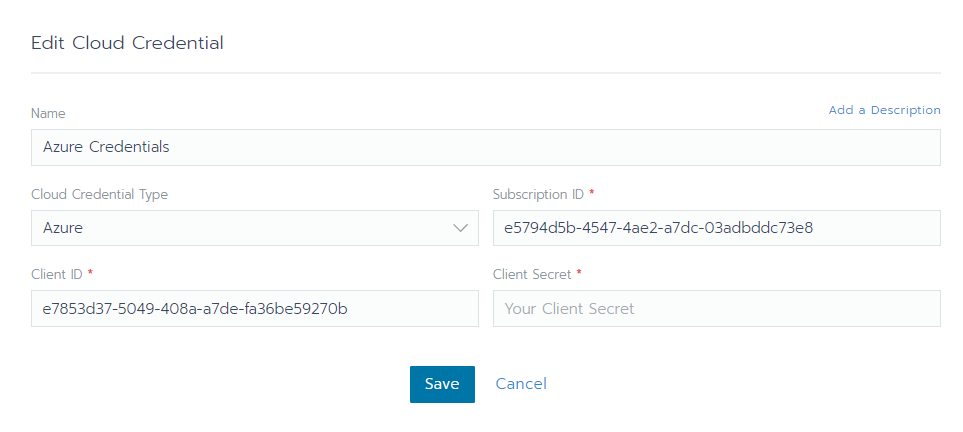
\includegraphics[width=\linewidth]{images/cloud-credentials.png}
\label{fig:cloudCredentials}
\end{figure}

\subsection{Node Templates}

Text. 

\begin{figure}[H]
\centering
\caption {Node Template}
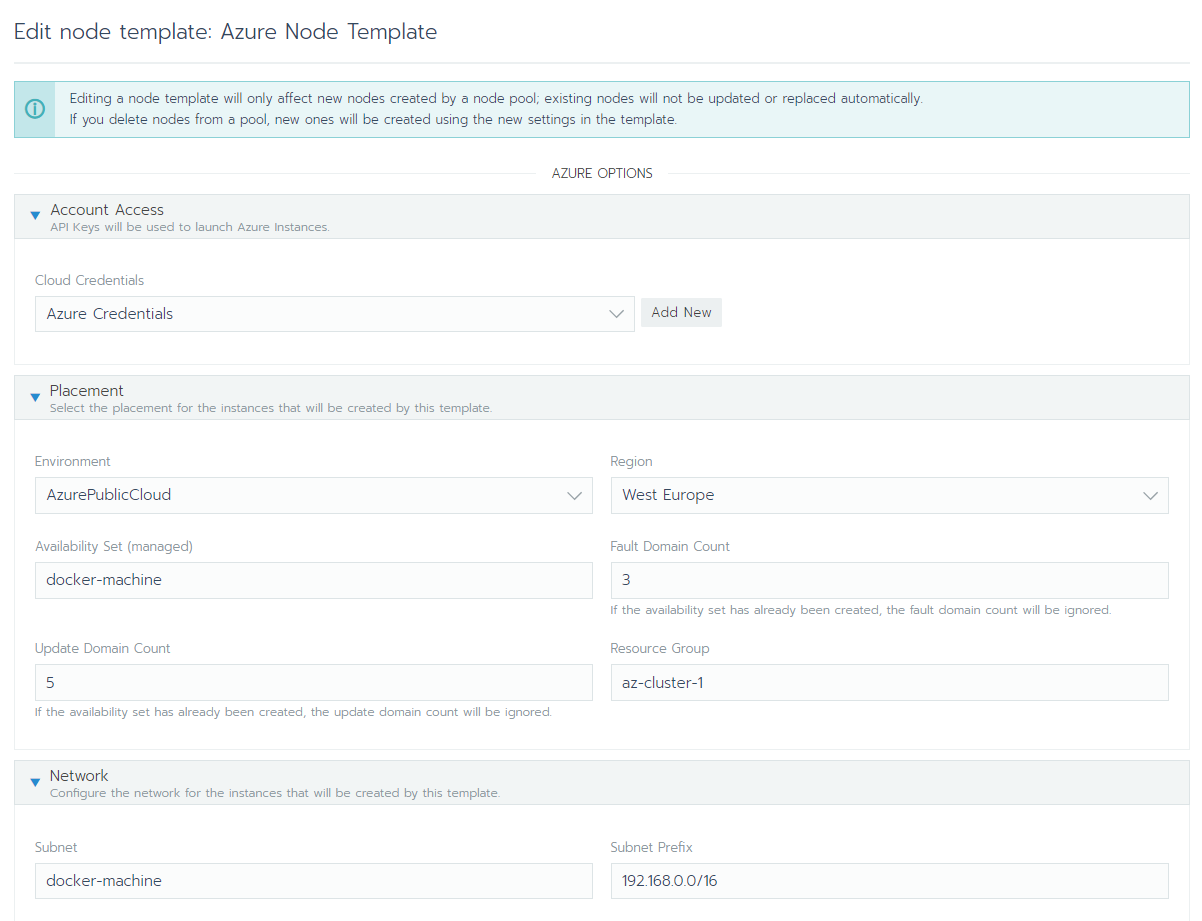
\includegraphics[width=\linewidth]{images/node-template.png}
\label{fig:nodeTemplate}
\end{figure}

\subsection{Cluster Templates}

Text. 

\begin{figure}[H]
\centering
\caption {Cluster Template}
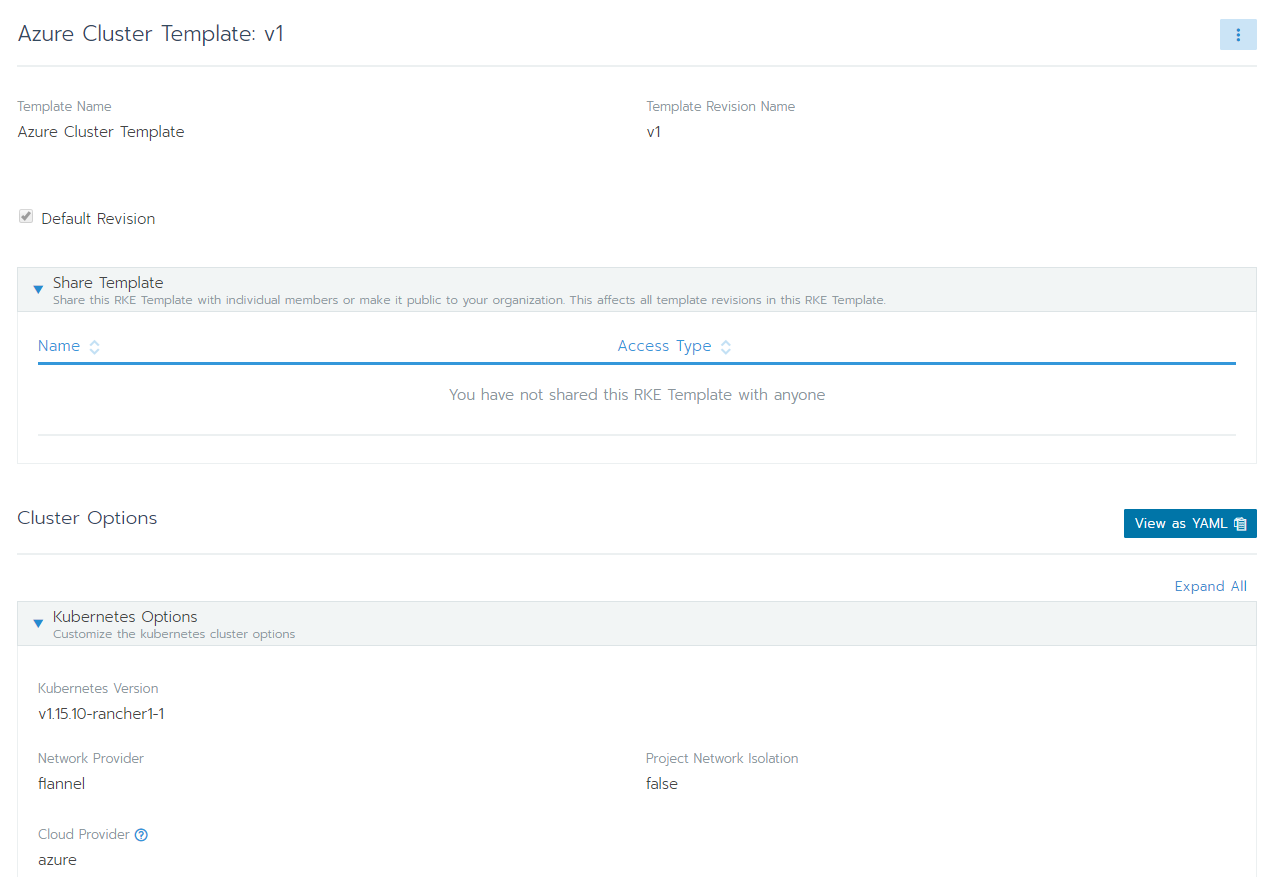
\includegraphics[width=\linewidth]{images/cluster-template.png}
\label{fig:clusterTemplate}
\end{figure}

\subsection{Kubernetes Cluster}

Text. 

\begin{figure}[H]
\centering
\caption {Kubernetes Cluster}
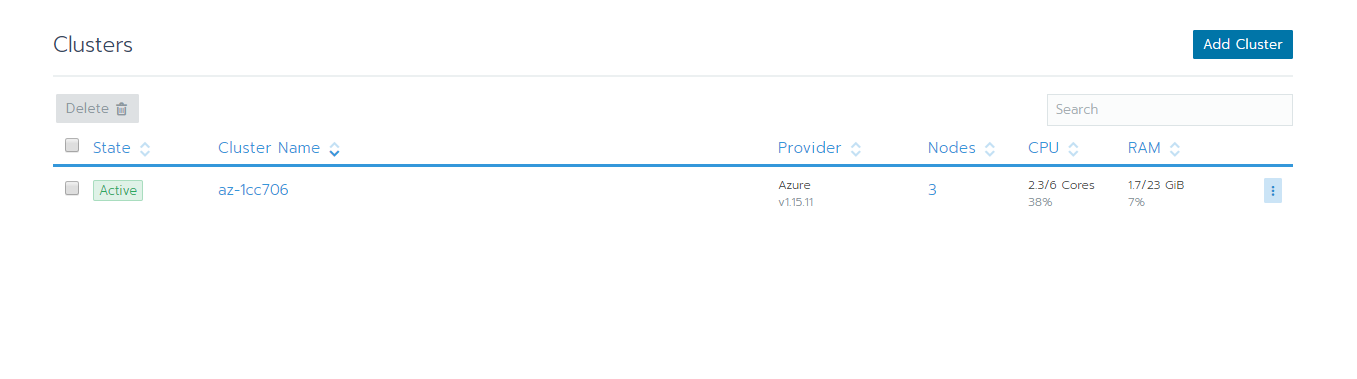
\includegraphics[width=\linewidth]{images/cluster-overview.png}
\label{fig:clusterOverview}
\end{figure}

